\chapter{Trees}\label{ch:trees}

Lists are linear: each element has one successor. \textbf{Trees} allow each
node to have several children, which models hierarchies (file systems,
organization charts), arithmetic expressions, and efficient search structures.

\section{Terminology}
A tree consists of \textbf{nodes}. One node is the \textbf{root}; every other
node has exactly one \textbf{parent}. Nodes with no children are
\textbf{leaves}. The \textbf{subtree} rooted at a node contains it and all its
descendants. The \textbf{depth} of a node is the number of edges from the
root; the \textbf{height} of a tree is the maximum depth of a leaf (conventions
differ by one; CS 135 often counts nodes on the longest root-to-leaf path).

\section{Binary trees}
Each node has at most two children, a left and a right subtree, either of
which may be empty.

\begin{lstlisting}[style=racket]
(define-struct node (key left right))
;; A Node is a (make-node Num BT BT)

;; A binary tree (BT) is one of:
;; * empty
;; * Node
\end{lstlisting}

\paragraph{Template.} Two self-references, so two recursive calls:
\begin{lstlisting}[style=racket]
;; bt-template: BT -> Any
(define (bt-template t)
  (cond [(empty? t) ...]
        [else (... (node-key t) ...
                   (bt-template (node-left t)) ...
                   (bt-template (node-right t)) ...)]))
\end{lstlisting}

\begin{lstlisting}[style=racket]
;; (size t) produces the number of nodes in t.
;; size: BT -> Nat
(define (size t)
  (cond [(empty? t) 0]
        [else (+ 1 (size (node-left t)) (size (node-right t)))]))

;; (height t) produces the number of nodes on a longest root-leaf path.
;; height: BT -> Nat
(define (height t)
  (cond [(empty? t) 0]
        [else (add1 (max (height (node-left t)) (height (node-right t))))]))

(define t1 (make-node 5 (make-node 2 empty empty)
                        (make-node 9 (make-node 7 empty empty) empty)))
(check-expect (size t1) 4)
(check-expect (height t1) 3)
\end{lstlisting}

\section{Binary search trees}

\begin{definition}[BST ordering property]
A binary tree is a \textbf{binary search tree} if for every node with key $k$,
every key in its left subtree is less than $k$ and every key in its right
subtree is greater than $k$.
\end{definition}

Tree \code{t1} above is a BST:
\begin{center}
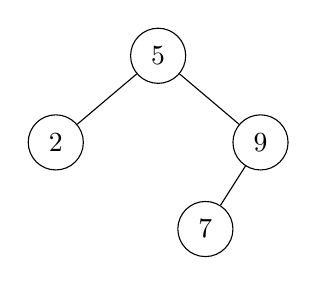
\begin{tikzpicture}[level distance=11mm,
  every node/.style={circle,draw,minimum size=7mm},
  level 1/.style={sibling distance=26mm},
  level 2/.style={sibling distance=14mm}]
  \node {5}
    child {node {2}}
    child {node {9} child {node {7}} child[missing]};
\end{tikzpicture}
\end{center}

For dictionaries, each node stores a key and a value:
\begin{lstlisting}[style=racket]
(define-struct bnode (key val left right))
;; A BST is one of:
;; * empty
;; * (make-bnode Num Str BST BST)
;;   requires: keys in left are < key, keys in right are > key
\end{lstlisting}

\subsection{Search}
The ordering property means only \emph{one} subtree need be searched:
\begin{lstlisting}[style=racket]
;; (search-bst k t) produces the value for key k in t, or false.
;; search-bst: Num BST -> (anyof Str false)
(define (search-bst k t)
  (cond [(empty? t) false]
        [(= k (bnode-key t)) (bnode-val t)]
        [(< k (bnode-key t)) (search-bst k (bnode-left t))]
        [else (search-bst k (bnode-right t))]))

(define dict (make-bnode 5 "five"
               (make-bnode 2 "two" empty empty)
               (make-bnode 9 "nine" empty empty)))
(check-expect (search-bst 9 dict) "nine")
(check-expect (search-bst 4 dict) false)
\end{lstlisting}
Condensed trace:
\begin{lstlisting}[style=racket]
(search-bst 9 dict)
=> (search-bst 9 (make-bnode 9 "nine" empty empty))   ; 9 > 5: go right
=> "nine"
\end{lstlisting}
The work is proportional to the height of the tree: about $\log_2 n$ if the
tree is balanced, but $n$ in the worst case (a ``stick'' created by inserting
keys in sorted order).

\subsection{Insertion}
\begin{lstlisting}[style=racket]
;; (insert-bst k v t) produces a BST like t with k mapped to v.
;; insert-bst: Num Str BST -> BST
(check-expect (insert-bst 1 "one" empty) (make-bnode 1 "one" empty empty))
(define (insert-bst k v t)
  (cond [(empty? t) (make-bnode k v empty empty)]
        [(= k (bnode-key t))
         (make-bnode k v (bnode-left t) (bnode-right t))]
        [(< k (bnode-key t))
         (make-bnode (bnode-key t) (bnode-val t)
                     (insert-bst k v (bnode-left t)) (bnode-right t))]
        [else
         (make-bnode (bnode-key t) (bnode-val t)
                     (bnode-left t) (insert-bst k v (bnode-right t)))]))
\end{lstlisting}
Note this builds a \emph{new} tree; only the nodes along the search path are
reconstructed.

\subsection{Traversal}
An \textbf{in-order} traversal (left, root, right) of a BST lists keys in
sorted order:
\begin{lstlisting}[style=racket]
;; bst->list: BST -> (listof Num)
(define (bst->list t)
  (cond [(empty? t) empty]
        [else (append (bst->list (bnode-left t))
                      (list (bnode-key t))
                      (bst->list (bnode-right t)))]))
\end{lstlisting}

\section{Evaluation (expression) trees}
An arithmetic expression such as $2 \times (3 + 4)$ is naturally a tree with
operators at internal nodes and numbers at leaves; the tree structure makes
the order of operations explicit, so no parentheses or precedence rules are
needed.

\begin{lstlisting}[style=racket]
(define-struct binode (op arg1 arg2))
;; A BinExp is one of:
;; * Num
;; * (make-binode (anyof '* '+ '/ '-) BinExp BinExp)

;; (eval-bin ex) produces the value of the expression ex.
;; eval-bin: BinExp -> Num
(check-expect (eval-bin 5) 5)
(check-expect (eval-bin (make-binode '* 2 (make-binode '+ 3 4))) 14)
(define (eval-bin ex)
  (cond [(number? ex) ex]
        [else (apply-op (binode-op ex)
                        (eval-bin (binode-arg1 ex))
                        (eval-bin (binode-arg2 ex)))]))

;; apply-op: Sym Num Num -> Num
(define (apply-op op a b)
  (cond [(symbol=? op '*) (* a b)]
        [(symbol=? op '+) (+ a b)]
        [(symbol=? op '/) (/ a b)]
        [(symbol=? op '-) (- a b)]))
\end{lstlisting}

\section{General trees and mutual recursion}
If an operator may have any number of arguments, as in Racket itself
(\code{(+ 1 2 3 4)}), a node holds a \emph{list} of subtrees. The data
definitions become \textbf{mutually recursive}:

\begin{lstlisting}[style=racket]
(define-struct opnode (op args))
;; An AExp is one of:
;; * Num
;; * (make-opnode (anyof '* '+) (listof AExp))
\end{lstlisting}
Here \code{AExp} refers to \code{(listof AExp)} and that list type refers back
to \code{AExp}. The templates are likewise mutually recursive --- one function
per type:

\begin{lstlisting}[style=racket]
;; aexp-template: AExp -> Any
(define (aexp-template ex)
  (cond [(number? ex) ...]
        [else (... (opnode-op ex) ...
                   (listof-aexp-template (opnode-args ex)) ...)]))

;; listof-aexp-template: (listof AExp) -> Any
(define (listof-aexp-template exlist)
  (cond [(empty? exlist) ...]
        [else (... (aexp-template (first exlist)) ...
                   (listof-aexp-template (rest exlist)) ...)]))
\end{lstlisting}

\begin{lstlisting}[style=racket]
;; (eval ex) produces the value of ex.
;; eval: AExp -> Num
(check-expect (eval (make-opnode '+ (list 1 (make-opnode '* (list 2 3 4)))))
              25)
(define (eval ex)
  (cond [(number? ex) ex]
        [else (apply (opnode-op ex) (opnode-args ex))]))

;; (apply f exlist) applies operator f to the values of exlist.
;; apply: Sym (listof AExp) -> Num
(define (apply f exlist)
  (cond [(empty? exlist) (cond [(symbol=? f '*) 1] [else 0])]
        [(symbol=? f '*) (* (eval (first exlist)) (apply f (rest exlist)))]
        [else (+ (eval (first exlist)) (apply f (rest exlist)))]))
\end{lstlisting}
The base case uses the identity of each operator: the empty sum is 0 and the
empty product is 1. (These names clash with built-ins in Intermediate
Student; rename to \code{my-eval}/\code{my-apply} there.)

\subsection{Condensed trace}
\begin{lstlisting}[style=racket]
(eval (make-opnode '+ (list 1 (make-opnode '* (list 2 3)))))
=> (apply '+ (list 1 (make-opnode '* (list 2 3))))
=> (+ (eval 1) (apply '+ (list (make-opnode '* (list 2 3)))))
=> (+ 1 (apply '+ (list (make-opnode '* (list 2 3)))))
=> (+ 1 (+ (eval (make-opnode '* (list 2 3))) (apply '+ empty)))
=> (+ 1 (+ (apply '* (list 2 3)) (apply '+ empty)))
=> (+ 1 (+ (* 2 (* 3 (apply '* empty))) (apply '+ empty)))
=> (+ 1 (+ (* 2 (* 3 1)) 0))
=> 7
\end{lstlisting}

\section{Nested lists and leaf-labelled trees}
A nested list such as \code{'(1 (2 3) ((4)))} is a tree whose leaves are the
numbers:
\begin{lstlisting}[style=racket]
;; A Nested-List-Num is one of:
;; * empty
;; * (cons Num Nested-List-Num)
;; * (cons Nested-List-Num Nested-List-Num)

;; (flatten lst) produces the numbers in lst in order, without nesting.
;; flatten: Nested-List-Num -> (listof Num)
(check-expect (flatten '(1 (2 3) ((4)))) '(1 2 3 4))
(define (flatten lst)
  (cond [(empty? lst) empty]
        [(number? (first lst)) (cons (first lst) (flatten (rest lst)))]
        [else (append (flatten (first lst)) (flatten (rest lst)))]))
\end{lstlisting}

\section{Summary}
\begin{itemize}
  \item Binary trees: two self-references, so two recursive calls in the template.
  \item BSTs: the ordering property lets search and insert follow one path; time proportional to height.
  \item Expression trees: operators at internal nodes, numbers at leaves; evaluation is a recursive traversal.
  \item General trees use a list of children, producing mutually recursive data definitions and templates.
\end{itemize}
